
\documentclass{article}
\usepackage{graphicx}
\usepackage{geometry}
\geometry{margin=1in}
\title{F1 Monaco 2024 Data Analysis}
\author{ F1-ML Pipeline }
\date{ June 24, 2025 }
\begin{document}
\maketitle

\section*{Introduction}
This report provides an automated analysis of Formula 1 lap data for the Monaco 2024 Grand Prix. It includes visualizations and interpretations generated by the F1-ML pipeline.


\section*{ Lap Time Distribution }
\begin{figure}[h!]
    \centering
    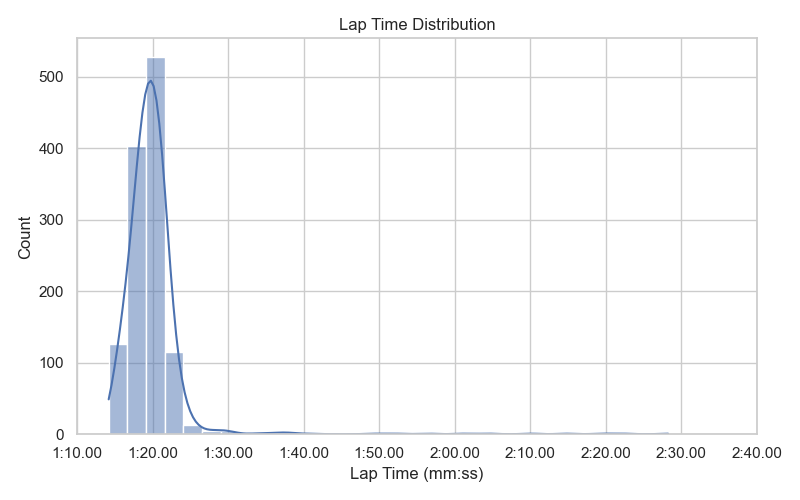
\includegraphics[width=0.8\textwidth]{ data/processed/2024/Monaco Grand Prix/lap_time_distribution.png }
    \caption{ Lap Time Distribution }
\end{figure}

\textbf{Interpretation:} Most lap times cluster around the mean, with a few slower laps (possibly due to pit stops or incidents).


\section*{ Lap Time vs. Position }
\begin{figure}[h!]
    \centering
    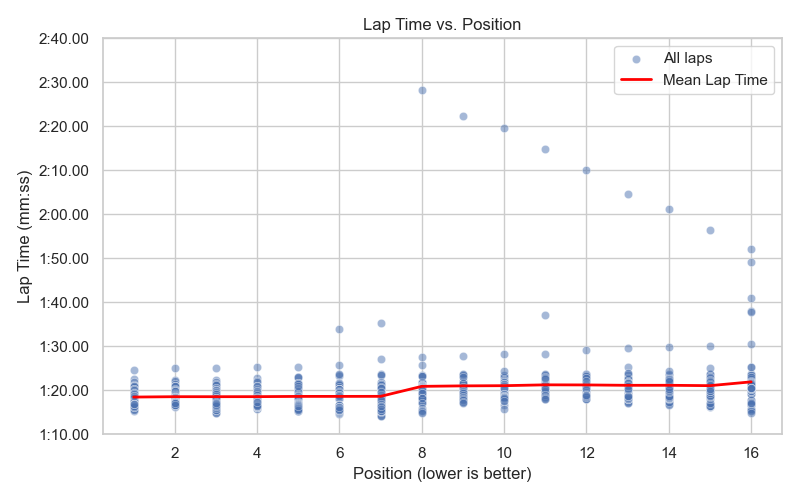
\includegraphics[width=0.8\textwidth]{ data/processed/2024/Monaco Grand Prix/lap_time_vs_position.png }
    \caption{ Lap Time vs. Position }
\end{figure}

\textbf{Interpretation:} Drivers in better positions (closer to 1) tend to have faster lap times, as expected. The red line shows the mean lap time for each position.


\section*{ Average Lap Time per Team }
\begin{figure}[h!]
    \centering
    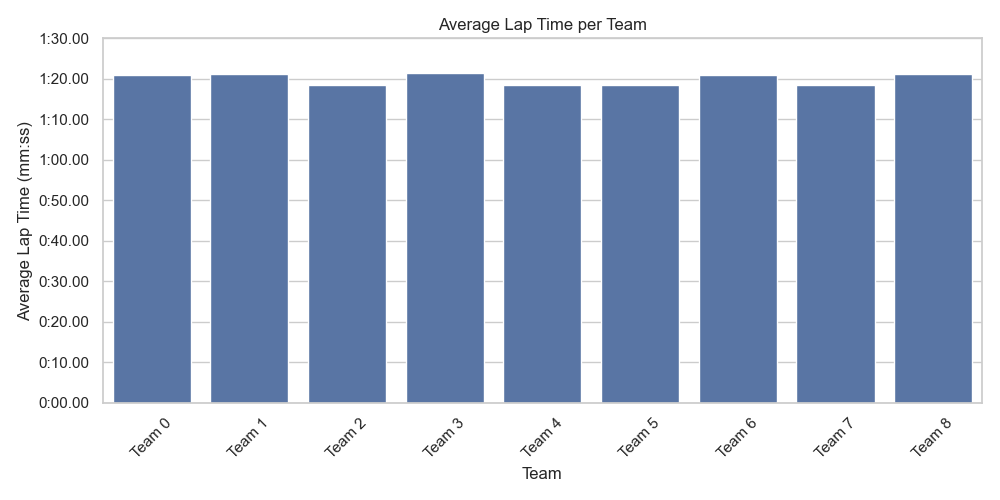
\includegraphics[width=0.8\textwidth]{ data/processed/2024/Monaco Grand Prix/avg_lap_time_per_team.png }
    \caption{ Average Lap Time per Team }
\end{figure}

\textbf{Interpretation:} Teams with lower average lap times are generally more competitive. Note: Some teams may be missing due to incidents.


\section*{ Lap Time Progression for 5 num16 }
\begin{figure}[h!]
    \centering
    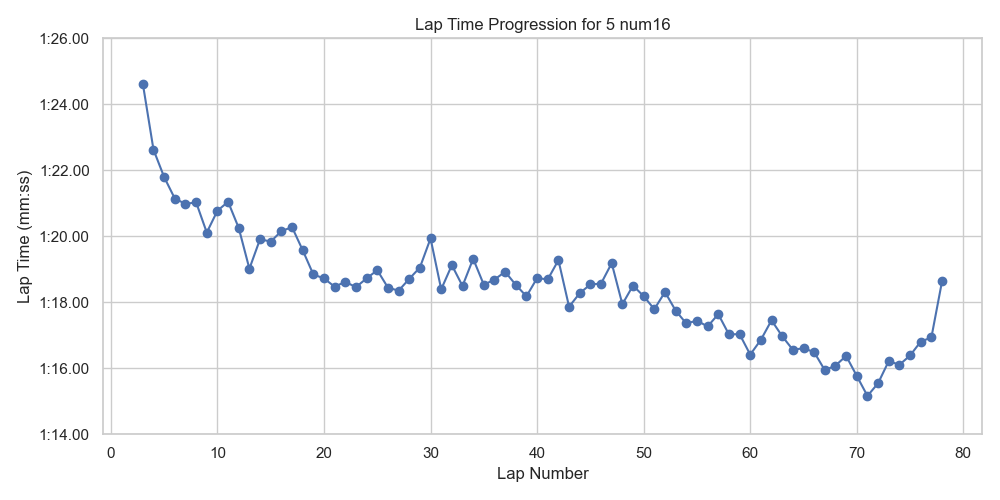
\includegraphics[width=0.8\textwidth]{ data/processed/2024/Monaco Grand Prix/lap_time_progression_driver_5_num16.png }
    \caption{ Lap Time Progression for 5 num16 }
\end{figure}

\textbf{Interpretation:} This shows how lap times change for 5 num16 over the race. Dips may indicate pit stops or faster laps.



\end{document}